\documentclass[11pt]{article}

\usepackage[left=0.75in, right=0.75in, top=0.75in, bottom=0.75in]{geometry}
\usepackage{layout}
\usepackage{ucs}
\usepackage[utf8x]{inputenc}
\usepackage{titlesec}
\usepackage{graphicx}
\usepackage{amssymb}
\usepackage{amsmath}
\usepackage{dsfont}
\usepackage{float}
\usepackage{caption}
\usepackage{subcaption}
\usepackage{array}



\title{\textbf{TS225 TP}\\Compte rendu}
\author{Maxime PETERLIN - \texttt{maxime.peterlin@enseirb-matmeca.fr}\\
Gabriel VERMEULEN - \texttt{gabriel@vermeulen.email} \\\\{ENSEIRB-MATMECA, Bordeaux}}
\date{20 octobre 2014}


\begin{document}

\maketitle
\tableofcontents

\newpage

\section{Différences entre la représentation RGB et $YC_{r}C_{b}$}
	
	\subsection{Equations de passage de l'espace RGB à l'espace $YC_{r}C_{b}$}

		Les équations sont les suivantes :
		\begin{align*}
			Y &= 0.299 R + 0.587 G + 0.114 B\\
			C_{b} &= 0.564(B-Y) + 128\\
			C_{r} &= 0.713(R-Y) + 128\\
		\end{align*}

	\subsection{Représentation de l'image pool.tif}

		On affiche l'image pool.tif suivant les différents canaux rouge (R), vert (G) et bleu (B), ainsi que la luminance (Y), la chrominance rouge ($C_{R}$) et la chrominance bleu $C_{B}$.\\

		\begin{figure}[h]
			\centering
			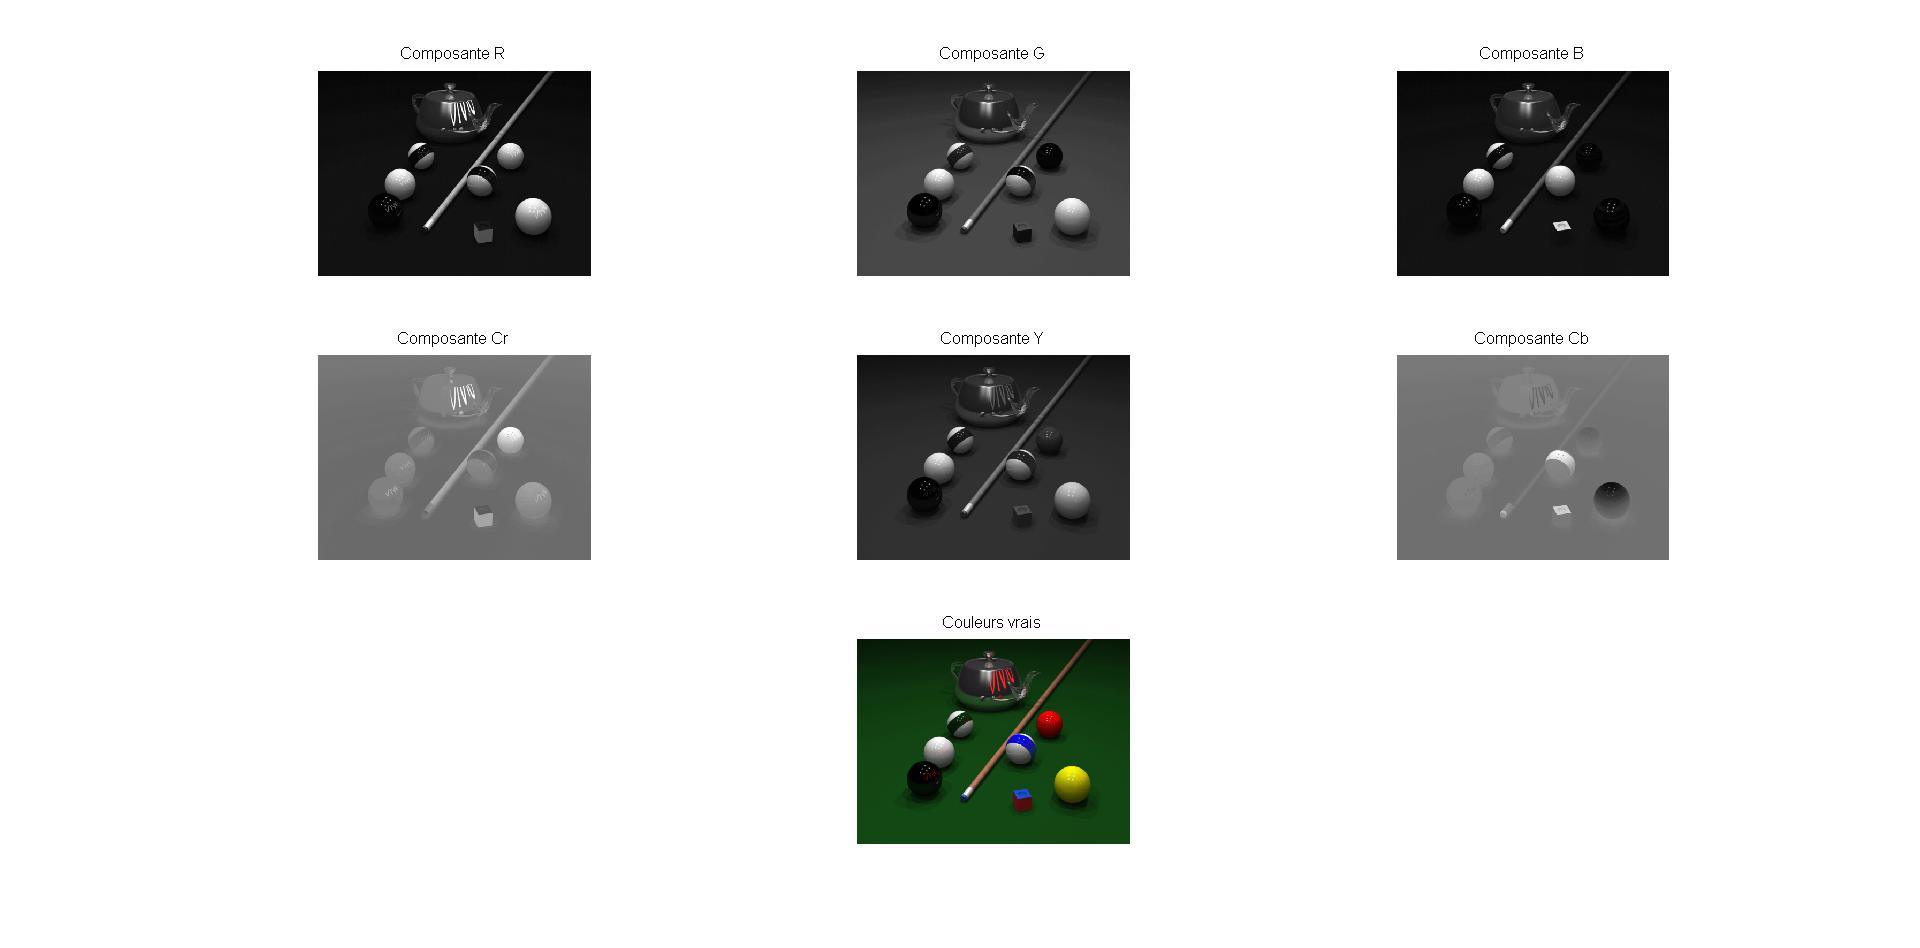
\includegraphics[scale=0.25]{img/rapport_img1-1.jpg}
			\caption{pool.tif}
			\label{Q412}
		\end{figure}

	\subsection{Intérêt de la représentation $YC_{r}C_{b}$}

		Sur les images qui représentent les composantes R, G et B, on remarque que la boule blanche apparaît blanche sur les trois images.\\
		\\
		Sur les images qui représentent les composantes Y, Cr, et Cb, on remarque que la boule blanche apparaît blanche uniquement sur l'image de la luminance. De plus, les boules ayant une couleur a forte dominante rouge ou bleu apparaîssent respectivement blanches sur les images de la crominance rouge ou bleu.\\




\section{Fusion des images background.jpg et foreground.jpg}
	
	Dans un premier temps, on va identifier la position des pixels correspondants au ciel grâce aux informations données par la chrominance bleu à l'aide d'un seuil égal à 145.\\

		\begin{figure}[h]
			\centering
			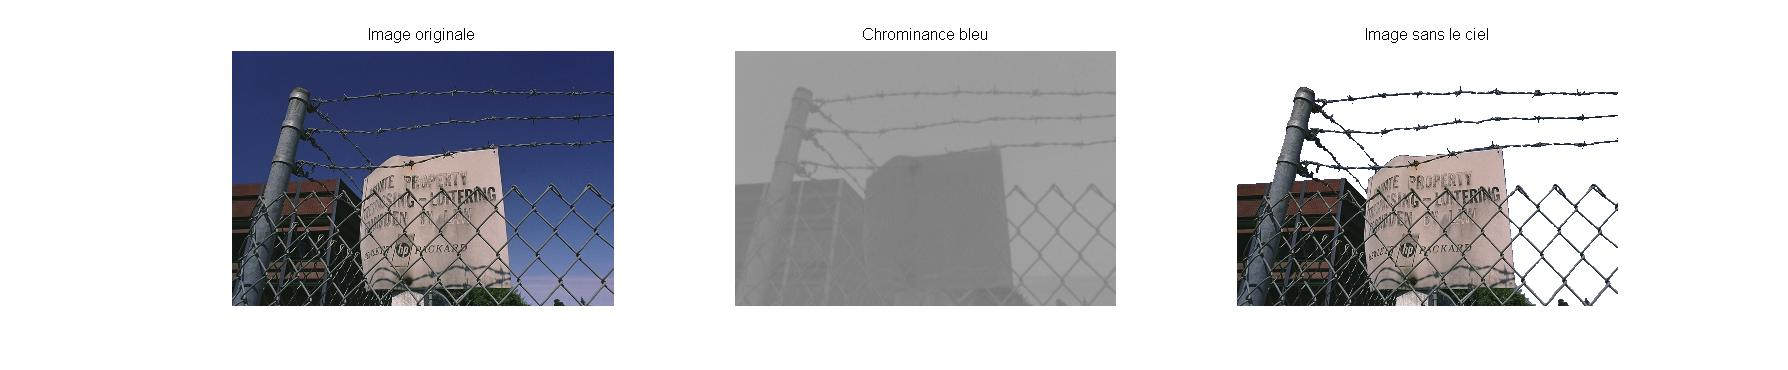
\includegraphics[scale=0.25]{img/rapport_img2-1.jpg}
			\label{Q412}
		\end{figure}

	Ensuite, en se basant sur ces positions, on remplace les pixels de foreground.jpg par les pixels de background.jpg, ce qui permet de fusionner les deux images.\\

		\begin{figure}[h]
			\centering
			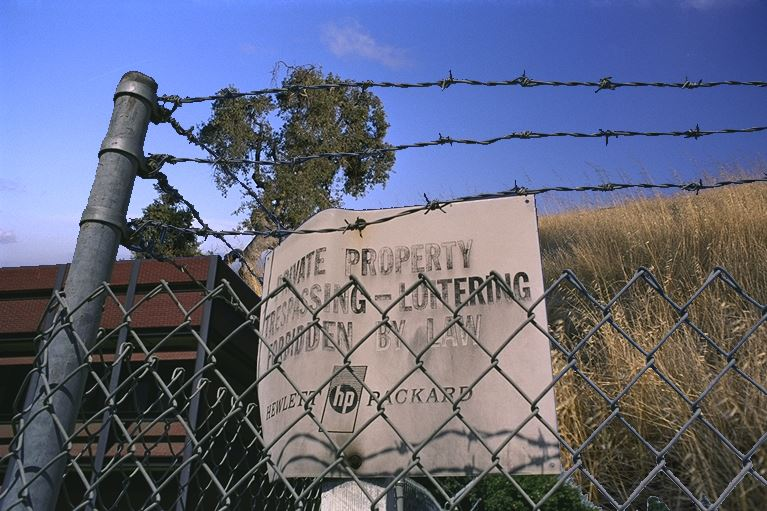
\includegraphics[scale=0.5]{img/rapport_img2-2.jpg}
			\caption{Fusion des images}
			\label{Q412}
		\end{figure}


\section{Pertinence de la représentation $YC_{r}C_{b}$}
	
	La représentation $YC_{r}C_{b}$ est ici plus adaptée qu'une representation RGB, car elle offre une meilleure représentation du rouge, du vert et du bleu. $YC_{r}C_{b}$ garde l'information sur les autres couleurs, ainsi un bleu pur (0, 0, 255) apparaîtra blanc sur la représentation $YC_{r}C_{b}$, alors que du violet (255, 0, 255) apparaitra grisé.


\end{document}
